\documentclass[final,hyperref={pdfpagelabels=false}]{beamer}
\usepackage{grffile}
\mode<presentation>{\usetheme{I6pd2}}
\usepackage[english]{babel}
\usepackage[utf8]{inputenc}
\usepackage{polski}
\usepackage{amsmath,amsthm, amssymb, latexsym}
%\usepackage{times}\usefonttheme{professionalfonts}  % obsolete
%\usefonttheme[onlymath]{serif}
\boldmath
\usepackage[orientation=portrait,size=a0,scale=1.4,debug]{beamerposter}
% change list indention level
% \setdefaultleftmargin{3em}{}{}{}{}{}


%\usepackage{snapshot} % will write a .dep file with all dependencies, allows for easy bundling

\usepackage{array,booktabs,tabularx}
\newcolumntype{Z}{>{\centering\arraybackslash}X} % centered tabularx columns
\newcommand{\pphantom}{\textcolor{ta3aluminium}} % phantom introduces a vertical space in p formatted table columns??!!

\listfiles

%%%%%%%%%%%%%%%%%%%%%%%%%%%%%%%%%%%%%%%%%%%%%%%%%%%%%%%%%%%%%%%%%%%%%%%%%%%%%%%%%%%%%%
\graphicspath{{figures/}}
 
\title{\huge PAAL: Practical Approximation Algorithm Library}
\author{Piotr Jaszkowski, Mateusz Machalica, Grzegorz Prusak and Łukasz Solak}
\institute[University of Warsaw]{The Faculty of Mathematics, Informatics and Mechanics, University of Warsaw, Warsaw, Poland}
\date[May 24, 2013]{May 24, 2013}

%%%%%%%%%%%%%%%%%%%%%%%%%%%%%%%%%%%%%%%%%%%%%%%%%%%%%%%%%%%%%%%%%%%%%%%%%%%%%%%%%%%%%%
\newlength{\columnheight}
\setlength{\columnheight}{105cm}


%%%%%%%%%%%%%%%%%%%%%%%%%%%%%%%%%%%%%%%%%%%%%%%%%%%%%%%%%%%%%%%%%%%%%%%%%%%%%%%%%%%%%%
\begin{document}
\begin{frame}
  \begin{columns}
    % ---------------------------------------------------------%
    % Set up a column 
    \begin{column}{.49\textwidth}
      \begin{beamercolorbox}[center,wd=\textwidth]{postercolumn}
        \begin{minipage}[T]{.95\textwidth}  % tweaks the width, makes a new \textwidth
          \parbox[t][\columnheight]{\textwidth}{ % must be some better way to set the the height, width and textwidth simultaneously
            % Since all columns are the same length, it is all nice and tidy.  You have to get the height empirically
            % ---------------------------------------------------------%
            % fill each column with content            
            \begin{block}{Introduction}
              \begin{itemize}
              \item Most face recognition approaches are sensitive to registration errors
                \begin{itemize}
                \item rely on a very good initial alignment and illumination
                \end{itemize}
              \item We propose/analyze:
                \begin{itemize}
                \item grid-based and dense extraction of local features
                \item block-based matching accounting for different\\
	                  viewpoints and registration errors
                \end{itemize}
              \end{itemize}              
            \end{block}
            \vfill
            \begin{block}{Feature Extraction}
              \begin{columns}
                \begin{column}{.55\textwidth}
                  \begin{itemize}
                  \item Interest point based feature extraction
                    \begin{itemize}
                    \item SIFT or SURF interest point detector
                    \item leads to a \alert{very sparse} description
                    \end{itemize}
                  \item Grid-based feature extraction
                    \begin{itemize}
                    \item overlaid regular grid
                    \item leads to a \alert{dense} description
                    \end{itemize}
                  \end{itemize}
                \end{column}
                \begin{column}{.44\textwidth}
                  \centering
                  \begin{tabularx}{\linewidth}{ZZZ}
                     Orig.
                     &
                     IP
                     &
                     Grid
                     \\
                    
\includegraphics[width=0.95\linewidth]{images/viola/m-012-1.png}
                    &
                    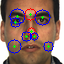
\includegraphics[width=0.95\linewidth]{images/viola/surf-64x64-ip/m-012-1.pngsurf.png}
                    &
                    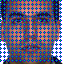
\includegraphics[width=0.95\linewidth]{images/viola/surf-64x64-4/m-012-1.pngsurf.png}
                    \\
                    
\includegraphics[width=0.95\linewidth]{images/viola/m-012-2.png}
                    &
                    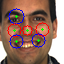
\includegraphics[width=0.95\linewidth]{images/viola/surf-64x64-ip/m-012-2.pngsurf.png}
                    &
                    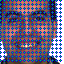
\includegraphics[width=0.95\linewidth]{images/viola/surf-64x64-4/m-012-2.pngsurf.png}
                    \\
                  \end{tabularx}
                \end{column}
              \end{columns}
              \vskip-1ex
            \end{block}
            \vfill
            \begin{block}{Feature Description}
              \begin{itemize}
              \item Scale Invariant Feature Transform (SIFT)
                \begin{itemize}
                \item 128-dimensional descriptor, histogram of gradients, scale invariant
                \end{itemize}
              \item Speeded Up Robust Features (SURF)
                \begin{itemize}
                \item 64-dimensional descriptor, histogram of gradients, scale invariant
                \end{itemize}
              \item face recognition: invariance w.r.t. rotation is often not necessary
                \begin{itemize}
                \item rotation dependent upright-versions U-SIFT, U-SURF-64, U-SURF-128
                \end{itemize}
              \end{itemize}
            \end{block}
            \vfill
            \begin{block}{Feature Matching}
              \begin{itemize}
              \item Recognition by Matching
                \begin{itemize}
                \item nearest neighbor matching strategy
                \item descriptor vectors extracted at keypoints in a test image $X$ are compared to all descriptor vectors extracted at keypoints from the reference images $Y_n, n=1,\cdots,N$ by the Euclidean distance
                \item decision rule:
                  \begin{align*}
                    X \rightarrow r(X) & = \arg \max_{c} \Big\{ \max_n \big\{ \sum_{x_i \in X} \delta(x_i,Y_{n,c})\big\} \Big\} 
                  \end{align*}
                \item additionally, a ratio constraint is applied in $\delta(x_i,Y_{n,c})$
                \end{itemize}
              \item Viewpoint Matching Constraints
                \begin{itemize}
                \item maximum matching: unconstrained
                \item grid-based matching: absolute box constraints
                \item grid-based best matching: absolute box constraints, overlapping
                \end{itemize}
              \item Postprocessing
                \begin{itemize}
                \item RANSAC-based outlier removal
                \item RANSAC-based system combination
                \end{itemize}
              \end{itemize}
            \end{block}
            \vfill
            \begin{block}{Matching Examples for the AR-Face and CMU-PIE Database}
              \begin{figure}
                \footnotesize
                \centering
                \begin{tabular}{p{.09\linewidth} | p{.12\linewidth} | p{.12\linewidth} | p{.12\linewidth} || p{.12\linewidth} | p{.12\linewidth} | p{.12\linewidth} | p{.09\linewidth} }
                  Feature
                  &
                  Maximum
                  & 
                  Grid
                  & 
                  Grid-Best
                  &
                  Maximum
                  & 
                  Grid
                  & 
                  Grid-Best
                  & 
                  Feature
                  \\
                  \hline
                  SIFT 
                  &
                  
\includegraphics[width=1.0\linewidth]{paper/bmvc09-surf/figures/matchings/arface-sift/maximum_m-005-17.pgm--w-052-4}
                  &
                  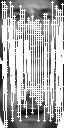
\includegraphics[width=1.0\linewidth]{paper/bmvc09-surf/figures/matchings/arface-sift/grid_m-005-17.pgm--m-005-4}
                  &
                  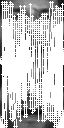
\includegraphics[width=1.0\linewidth]{paper/bmvc09-surf/figures/matchings/arface-sift/grid-best_m-005-17.pgm--m-005-4}
                  &
                  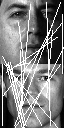
\includegraphics[width=1.0\linewidth]{paper/bmvc09-surf/figures/matchings/cmupie-surf/maximum_07-27-22.pgm--04-27-08}
                  &
                  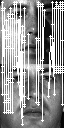
\includegraphics[width=1.0\linewidth]{paper/bmvc09-surf/figures/matchings/cmupie-surf/grid_07-27-22.pgm--07-27-08}
                  &
                  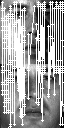
\includegraphics[width=1.0\linewidth]{paper/bmvc09-surf/figures/matchings/cmupie-surf/grid-best_07-27-22.pgm--07-27-08}
                  &
                  SURF
                  \\
                  \hline
                  U-SIFT
                  &
                  
\includegraphics[width=1.0\linewidth]{paper/bmvc09-surf/figures/matchings/arface-usift/maximum_m-005-17.pgm--w-052-4}
                  &
                  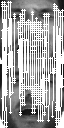
\includegraphics[width=1.0\linewidth]{paper/bmvc09-surf/figures/matchings/arface-usift/grid_m-005-17.pgm--m-005-4}
                  &
                  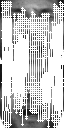
\includegraphics[width=1.0\linewidth]{paper/bmvc09-surf/figures/matchings/arface-usift/grid-best_m-005-17.pgm--m-005-4}
                  &
                  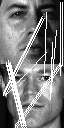
\includegraphics[width=1.0\linewidth]{paper/bmvc09-surf/figures/matchings/cmupie-usurf/maximum_07-27-22.pgm--04-27-08}
                  &
                  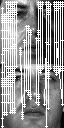
\includegraphics[width=1.0\linewidth]{paper/bmvc09-surf/figures/matchings/cmupie-usurf/grid_07-27-22.pgm--07-27-08}
                  &
                  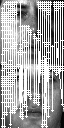
\includegraphics[width=1.0\linewidth]{paper/bmvc09-surf/figures/matchings/cmupie-usurf/grid-best_07-27-22.pgm--07-27-08}
                  &
                  U-SURF
                  \\
                  \hline
                \end{tabular}
              \end{figure}
              \begin{itemize}
              \item Matching results for the AR-Face (left) and the CMU-PIE database (right)
                \begin{itemize}
                \item maximum matching show false classification examples
                \item grid matchings show correct classification examples
                \item upright descriptor versions reduce the number of false matches
                \end{itemize}
              \end{itemize}
            \end{block}
          }
        \end{minipage}
      \end{beamercolorbox}
    \end{column}
    % ---------------------------------------------------------%
    % end the column

    % ---------------------------------------------------------%
    % Set up a column 
    \begin{column}{.49\textwidth}
      \begin{beamercolorbox}[center,wd=\textwidth]{postercolumn}
        \begin{minipage}[T]{.95\textwidth} % tweaks the width, makes a new \textwidth
          \parbox[t][\columnheight]{\textwidth}{ % must be some better way to set the the height, width and textwidth simultaneously
            % Since all columns are the same length, it is all nice and tidy.  You have to get the height empirically
            % ---------------------------------------------------------%
            % fill each column with content
            
            \begin{block}{Databases}
              \begin{columns}
                \begin{column}{.6\textwidth}
                  \begin{itemize}
                  \item AR-Face 
                    \begin{itemize}
                    \item variations in illumination
                    \item many different facial expressions
                    \end{itemize}
                  \item CMU-PIE
                    \begin{itemize}
                    \item variations in illumination (frontal images from the illumination subset)
                    \end{itemize}
                  \end{itemize}
                \end{column}
                \begin{column}{.39\textwidth}
                  
\includegraphics[width=0.22\linewidth]{hanselmann-databases/arface/train/png/occlusions/arneutral/m-016-1}
                  \-
                  
\includegraphics[width=0.22\linewidth]{hanselmann-databases/arface/train/png/cropped/m-016-4}
                  \-
                  
\includegraphics[width=0.22\linewidth]{hanselmann-databases/arface/test/png/occlusions/ar1sun/m-016-8}
                  \-
                  
\includegraphics[width=0.22\linewidth]{hanselmann-databases/arface/test/png/occlusions/ar1scarf/m-016-11}
                  \vskip3ex

                  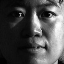
\includegraphics[width=0.22\linewidth]{hanselmann-databases/cmupie/test/png/cropped/00-27-02}
                  \-
                  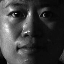
\includegraphics[width=0.22\linewidth]{hanselmann-databases/cmupie/test/png/cropped/00-27-17}
                  \-
                  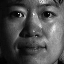
\includegraphics[width=0.22\linewidth]{hanselmann-databases/cmupie/test/png/cropped/00-27-18}
                  \-
                  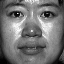
\includegraphics[width=0.22\linewidth]{hanselmann-databases/cmupie/test/png/cropped/00-27-20}
                \end{column}
              \end{columns}
            \end{block}
            \vfill
            \begin{block}{Results: Manually Aligned Faces}
              \begin{itemize}
              \item AR-Face: 110 classes, 770 train, 770 test
              \end{itemize}
              \vskip-0.5ex
              \begin{table}
                \centering
                \small
                \begin{tabular}{@{} p{.2\linewidth} p{.18\linewidth} p{.25\linewidth} r r r @{}}
                  \toprule 
                  Descriptor &  Extraction        & \multicolumn{1}{p{.2\linewidth}}{\# Features}           & \multicolumn{3}{c @{}}{Error Rates [\%]}         \\
                  \cmidrule(l){4-6}
                             &                    &                                                      & \multicolumn{1}{c}{Maximum} & \multicolumn{1}{c}{Grid} & \multicolumn{1}{c @{}}{Grid-Best} \\
                  \cmidrule(r){1-1}  \cmidrule(lr){2-2}   \cmidrule(lr){3-3}                               \cmidrule(lr){4-4}            \cmidrule(lr){5-5}         \cmidrule(l){6-6}  
                  SURF-64    & IPs                & \pphantom{1}64 $\times$ 5.6 (avg.)                    & 80.64     &  84.15  & 84.15     \\
                  SIFT       & IPs                & 128 $\times$ 633.78 (avg.)                           & 1.03      &  95.84  & 95.84      \\
                  \addlinespace
                  SURF-64    & 64x64-2 grid       & \pphantom{1}64 $\times$ 1024                          & 0.90      &  0.51   & 0.90      \\  
                  SURF-128   & 64x64-2 grid       & 128 $\times$ 1024                                    & 0.90      &  0.51   & 0.38       \\
                  SIFT       & 64x64-2 grid       & 128 $\times$ 1024                                    & 11.03     &  0.90   & 0.64       \\
                  \addlinespace
                  U-SURF-64  & 64x64-2 grid       & \pphantom{1}64 $\times$ 1024                          & 0.90      &  1.03   & 0.64      \\ 
                  U-SURF-128 & 64x64-2 grid       & 128 $\times$ 1024                                    & 1.55      &  1.29   & 1.03       \\ 
                  U-SIFT     & 64x64-2 grid       & 128 $\times$ 1024                                    & \textbf{0.25}  &  \textbf{0.25}   & \textbf{0.25}  \\
                  % \midrule
                  % \multicolumn{3}{l}{Modular PCA \cite{TanChen:subpatternPCA:Neurocomputing2005}}                         & 14.14 \\
                  % \multicolumn{3}{l}{Adaptively weighted Sub-Pattern PCA \cite{TanChen:subpatternPCA:Neurocomputing2005}} & 6.43  \\
                  % \multicolumn{3}{l}{DCT \cite{ekenel:LocalapFaceRecog:cvprbw2006}}                                       & 4.70  \\
                  \bottomrule
                \end{tabular}
              \end{table}

              \vskip1ex
              \begin{itemize}
              \item CMU-PIE: 68 classes, 68 train (``one-shot'' training), 1360 test
              \end{itemize}
              \vskip-0.5ex
              \begin{table}
                \centering
                \small
                \begin{tabular}{@{} p{.2\linewidth} p{.18\linewidth} p{.25\linewidth} r r r @{}}
                  \toprule 
                  Descriptor              &  Extraction    & \# Features                            & \multicolumn{3}{c @{}}{Error Rates [\%]}      \\
                  \cmidrule(l){4-6}
                                          &                    &                                    & \multicolumn{1}{c}{Maximum} & \multicolumn{1}{c}{Grid} & \multicolumn{1}{c @{}}{Grid-Best} \\
                  \cmidrule(r){1-1}  \cmidrule(lr){2-2}   \cmidrule(lr){3-3}                          \cmidrule(lr){4-4}            \cmidrule(lr){5-5}         \cmidrule(l){6-6}  
                  SURF-64    & IPs           & \pphantom{1}64 $\times$ 6.80 (avg.)                  & 93.95         & 95.21             & 95.21     \\  
                  SIFT       & IPs           & 128 $\times$ 723.17 (avg.)                           & 43.47         & 99.33             & 99.33     \\  
                  \addlinespace
                  SURF-64    & 64x64-2 grid  & \pphantom{1}64  $\times$ 1024                        &   13.41       &  4.12             &  7.82     \\
                  SURF-128   & 64x64-2 grid  & 128 $\times$ 1024                                    &  12.45        &  3.68             & 3.24      \\  
                  SIFT       &  64x64-2 grid & 128 $\times$ 1024                                    & 27.92         &  7.00             & 9.80      \\  
                  \addlinespace
                  U-SURF-64  & 64x64-2 grid  & \pphantom{1}64  $\times$ 1024                        & \textbf{3.83} &   \textbf{0.51}   & \textbf{0.66}    \\  
                  U-SURF-128 & 64x64-2 grid  & 128 $\times$ 1024                                    & 5.67          &  0.95             & 0.88      \\  
                  U-SIFT     & 64x64-2 grid  & 128 $\times$ 1024                                    & 16.28         &  1.40             & 6.41      \\
                  % \midrule
                  % \midrule
                  % \multicolumn{3}{l}{Spherical Harmonics \cite{ZhangSamaras:SphericalHarmonics:pami2006}}                              & 1.80 \\
                  % \multicolumn{3}{l}{Modeling Phase Spectra using GMM \cite{MitraSavvidesBrockwell:ModelingPhaseSpectra:lncs2005}}    & 12.83 \\
                  \bottomrule
                \end{tabular}
              \end{table}              
            \end{block}
            \vfill
            \begin{block}{Results: Unaligned Faces}
              \begin{columns}
                \begin{column}{.59\textwidth}
                  \begin{itemize}
                  \item Automatically aligned by Viola \& Jones
                  \end{itemize}
                  \vskip-0.5ex
                  \begin{table}
                    \centering
                    \small
                    \begin{tabular}{@{} p{.4\linewidth} r r @{}}
                      \toprule 
                      Descriptor  &      \multicolumn{2}{c @{}}{Error Rates [\%]}      \\
                      \cmidrule(l){2-3}   
                      &   AR-Face       & CMU-PIE  \\
                      \cmidrule(r){1-1}  \cmidrule(lr){2-2}  \cmidrule(l){3-3}  
                      SURF-64     &   5.97          & 15.32    \\ 
                      SURF-128    &   5.71          & 11.42    \\ 
                      SIFT        &   5.45          & 8.32     \\  
                      \addlinespace
                      U-SURF-64   &   5.32          & 5.52     \\  
                      U-SURF-128  &   5.71          & \textbf{4.86}  \\ 
                      U-SIFT      &   \textbf{4.15} & 8.99     \\  
                      \bottomrule
                    \end{tabular}
                  \end{table}
                \end{column}
                \begin{column}{.39\textwidth}                
                  \vskip-3ex
                  \begin{itemize}
                  \item Manually aligned faces 

                      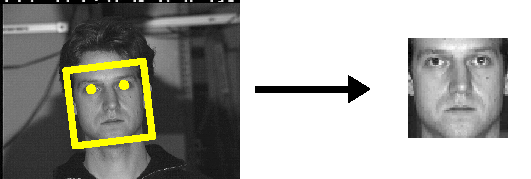
\includegraphics[width=0.9\linewidth]{hanselmann-thesis/slides/figures/alignment_cmu}

                  \item Unaligned faces 

                      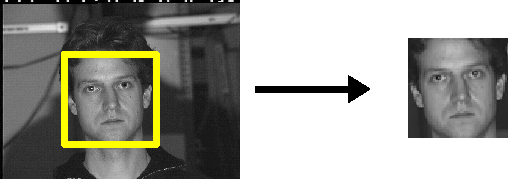
\includegraphics[width=0.9\linewidth]{hanselmann-thesis/slides/figures/unalignment_cmu}

                  \end{itemize}
                \end{column}
              \end{columns}
            \end{block}
            \vfill
            \begin{block}{Results: Partially Occluded Faces}
              \begin{itemize}
              \item AR-Face: 110 classes, 110 train (``one-shot'' training), 550 test
              \end{itemize}
              \vskip-0.5ex
              \begin{table}
                \small
                \centering
                \begin{tabular}{@{} l @{} r r r r r r@{}}
                  \toprule 
                  Descriptor          & \multicolumn{6}{c @{}}{Error Rates [\%]}                                                                 \\
                  \cmidrule(l){2-7}
                  & \textit{AR1scarf}  & \textit{AR1sun}  & \textit{ARneutral} & \textit{AR2scarf} & \textit{AR2sun}  & Avg. \\
                  \cmidrule(r){1-1}     \cmidrule(lr){2-2}   \cmidrule(lr){3-3} \cmidrule(lr){4-4}   \cmidrule(lr){5-5}  \cmidrule(lr){6-6}  \cmidrule(l){7-7} 
                  SURF-64             & 2.72             & 30.00          & 0.00                & 4.54            & 47.27      & 16.90 \\        
                  SURF-128            & 1.81             & 23.63          & 0.00                & 3.63            & 40.90      & 13.99 \\
                  SIFT                & 1.81             & 24.54          & 0.00                & 2.72            & 44.54      & 14.72 \\
                  \addlinespace
                  U-SURF-64           & 4.54             & 23.63          & 0.00                & 4.54            & 47.27      & 15.99 \\
                  U-SURF-128          & 1.81             & \textbf{20.00} & 0.00                & 3.63            & 41.81      & 13.45 \\
                  U-SIFT              & \textbf{1.81}    & 20.90          & \textbf{0.00}       & \textbf{1.81}   & \textbf{38.18} & \textbf{12.54} \\
                  \cmidrule(r){1-1}     \cmidrule(lr){2-2}   \cmidrule(lr){3-3} \cmidrule(lr){4-4}   \cmidrule(lr){5-5}  \cmidrule(lr){6-6}  \cmidrule(l){7-7}
                  U-SURF-128+R        & 1.81             & 19.09          & 0.00                & 3.63             & 43.63     & 13.63 \\
                  U-SIFT+R            & 2.72             & \textbf{14.54} & 0.00                & \textbf{0.90}    & 35.45     & 10.72 \\
                  U-SURF-128+U-SIFT+R &  \textbf{0.90}   & 16.36          & \textbf{0.00}       & 2.72             & \textbf{32.72} & \textbf{10.54} \\       
                  % \midrule 
                  % \midrule 
                  % DCT \cite{ekenel:facialocclusion:icb2009}, baseline%
                  % & 8.2              & 61.8           & 7.3                & 16.4            & 62.7       & 31.28 \\
                  % DCT \cite{ekenel:facialocclusion:icb2009}, realigned%
                  % & 2.7              & 1.8            & 0.0                & 6.4             & 4.5        & 3.08  \\
                  \bottomrule
                \end{tabular}
              \end{table}
            \end{block}
            \vfill
            \begin{block}{Conclusions}
              \begin{itemize}
              \item Grid-based local feature extraction instead of interest points
              \item Local descriptors:
                \begin{itemize}
                \item upright descriptor versions achieved better results
                \item SURF-128 better than SURF-64
                \end{itemize}
              \item System robustness: manually aligned/unaligned/partially occluded faces
                \begin{itemize}
                \item SURF more robust to illumination
                \item SIFT more robust to changes in viewing conditions
                \end{itemize}
              \item RANSAC-based system combination and outlier removal
              \end{itemize}
            \end{block}
          }
          % ---------------------------------------------------------%
          % end the column
        \end{minipage}
      \end{beamercolorbox}
    \end{column}
    % ---------------------------------------------------------%
    % end the column
  \end{columns}
  \vskip1ex
  %\tiny\hfill\textcolor{ta2gray}{Created with \LaTeX \texttt{beamerposter}  \url{http://www-i6.informatik.rwth-aachen.de/~dreuw/latexbeamerposter.php}}
  \tiny\hfill{Created with \LaTeX \texttt{beamerposter}  \url{http://www-i6.informatik.rwth-aachen.de/~dreuw/latexbeamerposter.php} \hskip1em}
\end{frame}
\end{document}


%%%%%%%%%%%%%%%%%%%%%%%%%%%%%%%%%%%%%%%%%%%%%%%%%%%%%%%%%%%%%%%%%%%%%%%%%%%%%%%%%%%%%%%%%%%%%%%%%%%%
%%% Local Variables: 
%%% mode: latex
%%% TeX-PDF-mode: t
%%% End:
